\documentclass[a0,landscape]{a0poster}

\usepackage[paper=a0paper, landscape, margin=2cm]{geometry}

\usepackage{multicol} % This is so we can have multiple columns of text side-by-side
\columnsep=100pt % This is the amount of white space between the columns in the poster
\columnseprule=1pt

\usepackage{tikz}

\usepackage{sectsty}
\sectionfont{\huge\selectfont}

\usepackage[scaled]{helvet}
\renewcommand\familydefault{\sfdefault} 
\usepackage[T1]{fontenc}

\usepackage{graphicx} % Required for including images
\usepackage{subfig}
\usepackage{booktabs} % Top and bottom rules for table
\usepackage[font=small,labelfont=bf]{caption} % Required for specifying captions to tables and figures
\usepackage{amsfonts, amsmath, amsthm, amssymb} % For math fonts, symbols and environments
\usepackage{wrapfig} % Allows wrapping text around tables and figures

\usepackage[hypcap=false]{caption}
\captionsetup{margin=0.5cm,font=large,labelfont=bf}
\captionsetup[subfloat]{margin=0.5cm,font=large,labelfont=bf}

\newenvironment{Figure}
  {\par\medskip\noindent\minipage{\linewidth}}
  {\endminipage\par\medskip}

\usepackage[hidelinks]{hyperref}

\usepackage{pgfplots}
\usepackage{pgfplotstable}
\pgfplotsset{compat=newest}
\usepgfplotslibrary{groupplots}

\definecolor{tableau_blue}{RGB}{31, 119, 180}
\definecolor{tableau_red}{RGB}{214, 39, 40}
\definecolor{tableau_green}{RGB}{44, 160, 44}

\begin{document}

\tikz[remember picture,overlay] \node[inner sep=0pt, anchor=north] at (current page.north){
\includegraphics[width=\paperwidth,height=12cm]{GreenBackground.pdf}};

\vspace{-1cm}
\begin{minipage}[t]{0.3\linewidth}
\vspace{0pt}

\includegraphics[width=0.9\textwidth]{UofALogo.pdf}
\end{minipage}
%
\begin{minipage}[t]{0.7\linewidth}
\vspace{0.75cm}
\color{white}
\veryHuge \textbf{\textsc{Redliner: An Activity Monitor for Manual Wheelchair Users}}\\[1cm]
\huge {Kenton Hamaluik, MSc, EIT\textsuperscript{1}, Zohreh Salimi, MSc\textsuperscript{2}, Martin Ferguson-Pell, PhD, C.Phys.\textsuperscript{3}}\\
\large \textsuperscript{1}\href{mailto:hamaluik@ualberta.ca}{hamaluik@ualberta.ca}, \textsuperscript{2}\href{mailto:zsalimi@ualberta.ca}{zsalimi@ualberta.ca}, \textsuperscript{3}\href{mailto:martin.ferguson-pell@ualberta.ca}{martin.ferguson-pell@ualberta.ca}\\
%\large \textsuperscript{1}Faculty of Rehabilitation Medicine, University of Alberta;\ \textsuperscript{2}Peter Lougheed Leadership College\\
\end{minipage}

\vspace{4cm}

\begin{multicols*}{3}
\large

\section*{Background}
\begin{minipage}[t]{0.5\columnwidth}
    \begin{itemize}
        \item Wheelchair users have a need for daily activity monitoring
            \begin{itemize}
                \item Manual wheelchair users are highly susceptible to repetitive stress injuries \cite{mercer06}
                \item Propulsion forces over 80\% of maximum capacity often result in injuries \cite{hills11}
            \end{itemize}
        \item Typical existing activity monitors (Fitbit\textsuperscript{\textregistered}, etc) \textbf{don't work} with manual wheelchair users
        \item SmartWheels are the gold standard \cite{asato93,cowan08}
            \begin{itemize}
                \item Prohibitively expensive for consumers
                \item Require chair modification (replacing the wheels)
            \end{itemize}
    \end{itemize}
\end{minipage}
\hspace{0.05\columnwidth}%
\begin{minipage}[t]{0.45\columnwidth}
    \begin{Figure}
        \centering
        \includegraphics[width=\linewidth]{photos/smartwheel.png}
        \captionof{figure}{A SmartWheel instrumented wheelchair wheel.}
        \label{fig:smartwheel}
    \end{Figure}
\end{minipage}

\section*{Objective}
\begin{itemize}
    \item Create an \textbf{inexpensive} activity monitor for \textbf{manual wheelchair users} which continuously monitors the following:
    \begin{itemize}
        \item Number of propulsion strokes
        \item Average travel velocity
        \item Amount of time spent active
        \item Estimated distance travelled
        \item Number of ``redline events''\textsuperscript{1}
    \end{itemize}
\end{itemize}
\textsuperscript{1} \textit{redline events} are instances of when the user's propulsion force exceeds 80\% of the maximal propulsion force they can generate, thus indicating potential for injury

\section*{Method}
\begin{minipage}[t]{0.45\columnwidth}
     \begin{Figure}
        \centering
        \includegraphics[width=0.75\linewidth]{photos/redliner_alpha.png}
        \captionof{figure}{Original Redliner prototype, assembled using breakout boards}
        \label{fig:redliner:alpha}
    \end{Figure}
\end{minipage}
\hspace{0.05\columnwidth}%
\begin{minipage}[t]{0.5\columnwidth}
    \begin{itemize}
        \item Utilize Newton's laws of motion to estimate propulsion force using kinematic data
        \item Create a simple prototype to perform the measurements for analysis
        \item Collect and compare synchronous propulsion data between SmartWheel and Redliner across varied terrain:
        \begin{itemize}
            \item Linoleum
            \item Grass
            \item Gravel
            \item Pavement
        \end{itemize}
    \end{itemize}
\end{minipage}

\section*{Results}
\begin{itemize}
    \item Velocity and acceleration data fro
\end{itemize}

\begin{Figure}
    \centering
    \begin{tikzpicture}
        \begin{groupplot}[group style={group size=1 by 2,
            horizontal sep=0pt,
            vertical sep=2cm}
        ]
            \nextgroupplot[
                width=0.8\linewidth,height=0.3\linewidth,
                xmin=0, xmax=26, ymin=-0.25, ymax=1.75,
                xtick={0,2,...,26}, ytick={0,0.4,...,1.6}, grid=both,
                axis lines=left,
                ylabel={Velocity, $v$, $\frac{\mathrm{m}}{\mathrm{s}}$}
            ]
            \addplot +[mark=noindent, line width=4pt, tableau_blue] table{data/assets/gravel_10_swv.dat}; \addlegendentry{\small\ SmartWheel}
            \addplot +[mark=noindent, line width=4pt, tableau_red] table{data/assets/gravel_10_rlv.dat}; \addlegendentry{\small\ Redliner}
            \nextgroupplot[
                width=0.8\linewidth,height=0.3\linewidth,
                xmin=0, xmax=26, ymin=-1.5, ymax=2.0,
                xtick={0,2,...,26}, ytick={-1.5,-1.0,...,2.0}, grid=both,
                axis lines=left,
                xlabel={Time, $t$ (s)}, ylabel={Acceleration, $a$, $\frac{\mathrm{m}}{\mathrm{s}^2}$}
            ]
            \addplot +[mark=noindent, line width=4pt, tableau_blue] table{data/assets/gravel_10_swa.dat};
            \addplot +[mark=noindent, line width=4pt, tableau_red] table{data/assets/gravel_10_rla.dat};
        \end{groupplot}
    \end{tikzpicture}
    \captionof{figure}{Velocity and acceleration traces for both SmartWheel and Redliner for 10 pushes on rough gravel.}
    \label{fig:10pushgravel}
\end{Figure}

\begin{Figure}
    \centering
    \begin{tikzpicture}
        \begin{axis}[
            legend cell align=left,
            width=0.8\linewidth,height=0.3\linewidth,
            xmin=0, xmax=26, ymin=-1.5, ymax=2.0,
            xtick={0,2,...,26}, ytick={-1.5,-1.0,...,2.0}, grid=both,
            axis lines=left,
            xlabel={Time, $t$ (s)}, ylabel={Acceleration, $a$, $\frac{\mathrm{m}}{\mathrm{s}^2}$}]
            \addplot +[mark=noindent, line width=4pt, tableau_blue] table{data/assets/gravel_10_rla.dat}; \addlegendentry{\small\ Acceleration}
            \addplot +[mark=noindent, line width=4pt, tableau_green] table{data/assets/gravel_10_pushes.dat}; \addlegendentry{\small\ Detected Pushes}
            \addplot +[mark=noindent, line width=4pt, tableau_red] table{data/assets/gravel_10_redline.dat}; \addlegendentry{\small\ Redline Events}
        \end{axis}
    \end{tikzpicture}
    \captionof{figure}{Acceleration, detected pushes, and redlines of 10 pushes on gravel as measured by Redliner.}
    \label{fig:10pushgravel_pushes}
\end{Figure}

\noindent
\begin{minipage}{\columnwidth}
\makeatletter
\newcommand{\@captype}{figure}
\makeatother
\centering
\subfloat[Second Redliner prototype version using a custom PCB built for further testing.]{%
  \includegraphics[width=0.45\linewidth]{photos/redliner_beta.png}%
  \label{fig:redliner_photo:beta}%
}\qquad%
\subfloat[Android app developed to interact with Redliner and upload data to a cloud dashboard.]{%
  \makebox[0.45\linewidth][c]{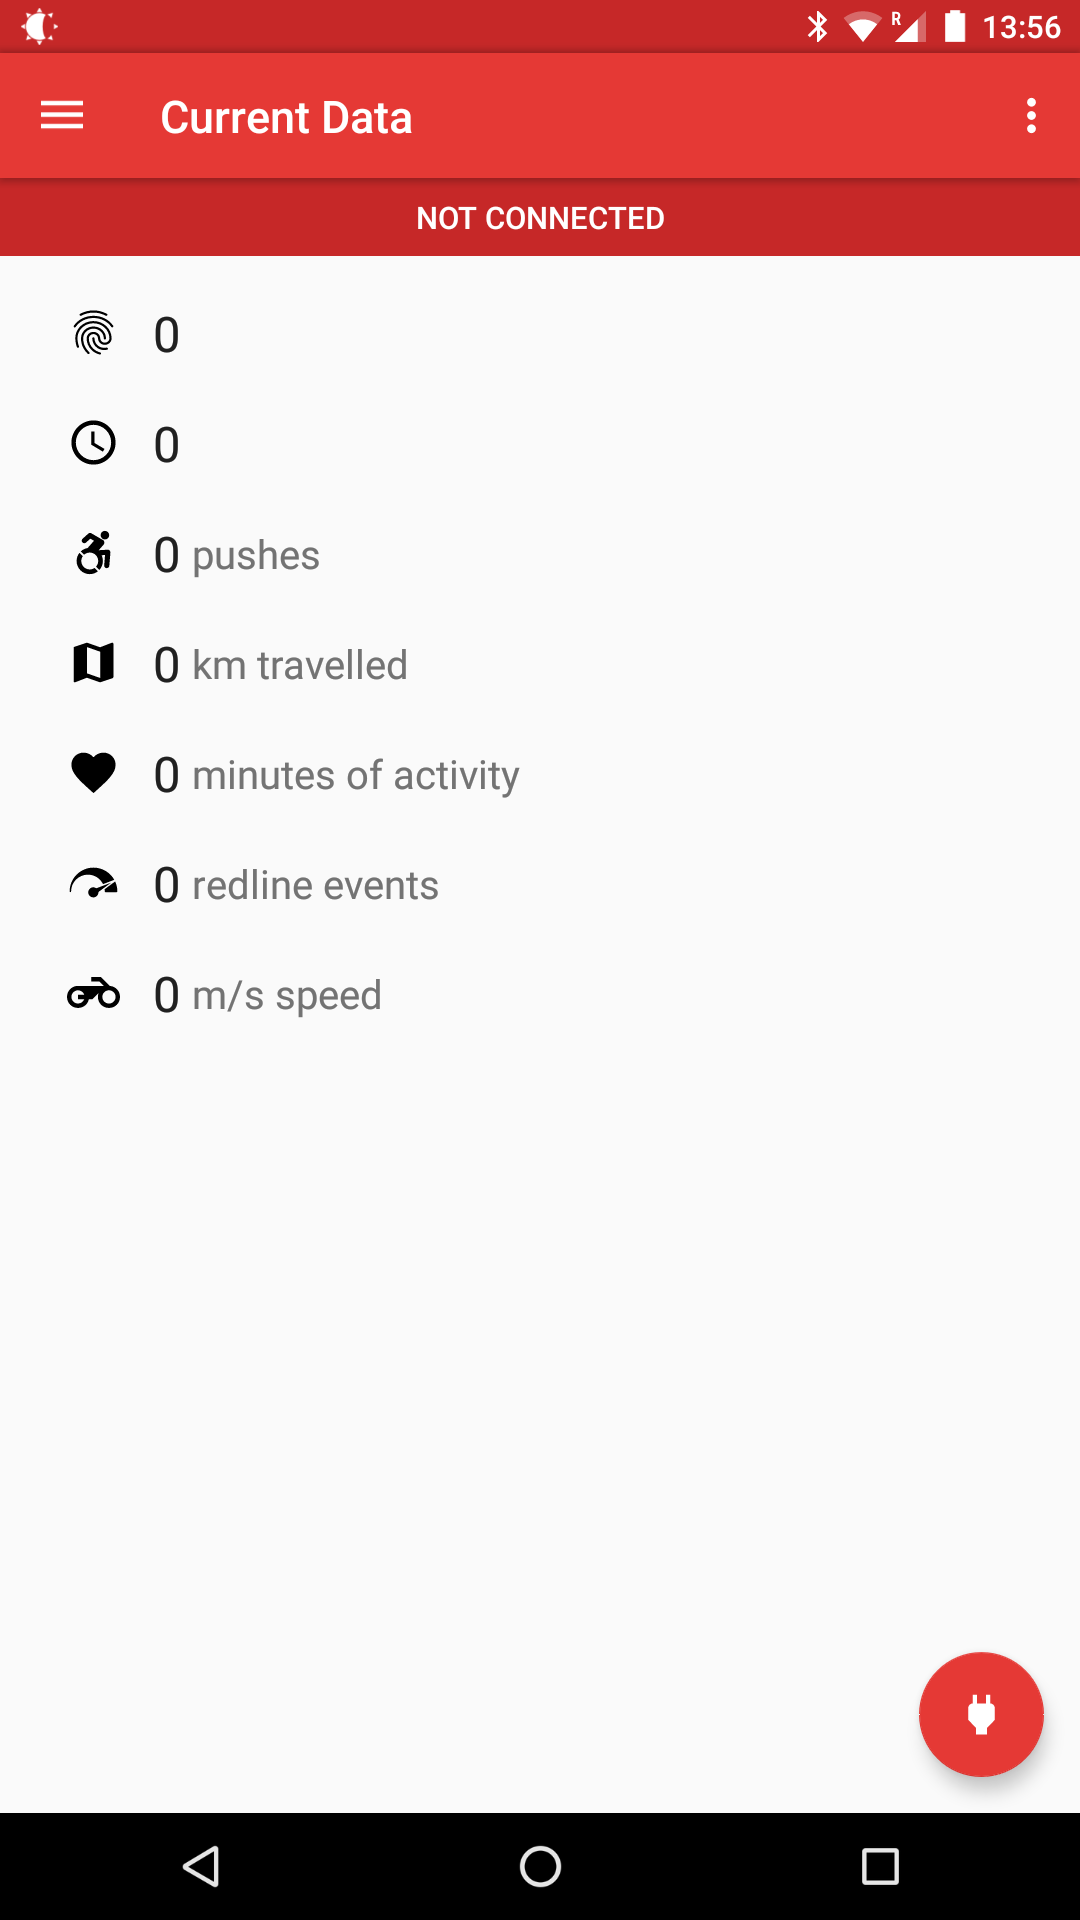
\includegraphics[height=0.45\linewidth]{photos/app_screenshot.png}}%
  \label{fig:redliner:app}%
}
\caption{Ongoing commercial development of Redliner}
\end{minipage}

\section*{Conclusions}
\begin{itemize}
    \item Redliner is a new activity monitor for manual wheelchair users
    \item Redliner has been validated against expensive SmartWheel devices
    \item Redliner is moving forward as a commercial entity to produce and sell the devices
\end{itemize}

\small
\nocite{*}
\bibliographystyle{unsrt}
\bibliography{sources}

\section*{Acknowledgements}
Funding for this work was provided for by the University of Alberta, Telus, Mitacs Accelerate Program, and Redliner Inc.

\end{multicols*}
\end{document}
